%%==================================================
%% ch2.tex for BIT Master Thesis
%% modified by yang yating
%% version: 0.5
%% last update: April 25th, 2017
%%==================================================

\chapter{模板使用}
\label{chap:textStructure}

本章的目的是介绍\LaTeX{}的文本控制流程,介绍学位论文中各章节分布以及模板内部组成,以及章节内的交叉引用问题,用户可以根据自身对\LaTeX{}的熟悉程度适当地略过阅读。在了解了本章的内容后,用户即可通过文本内容的粘贴和复制,快速实现生成一个格式满足基本需求的学位论文。

以硕士模板BIT-thesis-template-grd为例,文件布局如图 \ref{layout-master} 所示。 

\begin{lstlisting}[basicstyle=\small\ttfamily,caption={BIT-thesis-template-grd 模板文件布局},label=layout-master,numbers=none]
  ├── demo.tex              主控文件
  ├── demo.pdf              生成的论文pdfBIT-thesis-template-grd
  ├── BIT-thesis-grd.cls    格式控制文件
  ├── GBT7714-2005NLang.bst 参考文献格式控制文件
  ├── chapters              章节文件夹
  │   ├── abstract.tex       摘要
  │   ├── chapter01.tex      第一章
  │   ├── conclusion.tex     总结
  │   ├── app1.tex           附录A
  │   ├── pub.tex            攻读学位期间发表论文与研究成果清单
  │   └── thanks.tex         致谢
  ├── figures               图片文件夹
  │   └── figure1.png   
  ├── reference             参考文献文件夹
  │   └── chap1.bib
  ├── BIT-thesis-run.cmd    运行脚步cmd
  └── BIT-thesis-run.sh     运行脚本sh
  
      
\end{lstlisting}

\section{认识模板组成}

\subsection{格式控制文件}
\label{sec:format}

格式控制文件控制着论文的表现形式,包括以下两个文件:BIT-thesis-grd.cls 和 GBT7714-2005NLang.bst。
其中,``.cls''控制论文主体格式,``.bst''控制参考文献条目的格式,

一般用户可以``忽略''格式控制文件的存在。因为该文件已经按照《北京理工大学博士、硕士学位
论文撰写规范》进行了修改。有其他格式修改的需要,参见第\ref{sec:thesisformat}章。


\subsection{主控文件~demo.tex}
\label{sec:demotex}

主控文件~demo.tex~的作用就是将分散在多个文件中的内容``整合''成一篇完整的论文。
使用这个模板撰写学位论文时,学位论文内容和素材会被``拆散''到各个文件中:
譬如各章正文、各个附录、各章参考文献等等。
在~demo.tex~中通过``include''命令将论文的各个部分包含进来,从而形成一篇结构完成的论文。
封面页中的论文标题、作者等中英文信息,也是在~demo.tex~中填写。也可以在demo.tex中按照自己的需要引入一些的宏包
\footnote{一般只有当你需要在文档中使用那个宏包时,才需要在导言区中用~usepackage~引入该宏包。如若不然,通过usepackage引入一大堆不被用到的宏包,必然是一场灾难。由于一开始没有一致的设计目标,\LaTeX~ 的各宏包几乎都是独立发展起来的,因重定义命令导致的宏包冲突屡见不鲜。}。

大致而言,在主控文件~demo.tex~中,只需要留意文章有哪些章节以及各章参考文
献内容,不需要具体关注每一章里面的具体内容。需要注意,处理文档时所有的操作命令
{}\cndash{}xelatex, bibtex等,都是作用在~demo.tex~上,而\emph{不是}后面这
些``分散''的文件,请参考\ref{sec:process}小节。

若使用\textbf{硕士论文模板},请在~demo.tex~中~\verb|\documentclass|~命令采用~master~选项;若使用\textbf{博士论文模板},请使用~doctor~选项。同理,单页打印使用~oneside~选项,双面打印使用~twoside~选项。

文章各部分安排如下:
\begin{itemize}
\item ~\verb|\maketitle|~ : 中文封面
\item ~\verb|\makeInfo|~ : 中文信息
\item ~\verb|\makeEnglishInfo|~ : 英文信息
\item ~\verb|\makeVerticalTitle|~ : 打印竖排论文题目
\item ~\verb|\makeDeclareOriginal|~ : 论文原创性声明和使用授权
\item ~\verb|%%==================================================
%% abstract.tex for BIT Master Thesis
%% modified by yang yating
%% version: 0.1
%% last update: Dec 25th, 2016
%%==================================================

\begin{abstract}

本文主要的研究内容为固定翼无人机紧密编队控制器设计。该控制器以固定翼无人机编队的领从方法(leader-follower method)为基础,并考虑
内环的姿态驾驶仪的控制输入量,完成从编队误差量到姿态控制输入量的计算。
初步设计完成之后,再从无人机的动力学模型出发,使用MATLAB/Simulink等数学仿真工具研究控制器设计的稳定性以及动态特性。
其次选取合适的无人机飞行平台,飞行控制硬件并编写控制程序,完成飞行实验验证。完成编队控制器的参数参数整定之后,将实验的结果与仿真结果相对比,
最后,使用改进后的编队控制器完成双机编队任务,研究编队过程中的空气动力效果问题,
即研究此尺寸无人机编队群对提高整体飞行效率的作用。
%TODO:这里的研究目的要针对研究情况改写。
%({\color{blue}{摘要是一篇具有独立性和完整性的短文,应概括而扼要地反映出本论文的主要内容。包括研究目的、研究方法、研究结果和结论等,特别要突出研究结果和结论。中文摘要力求语言精炼准确,硕士学位论文摘要建议500$\sim$800字,博士学位论文建议1000$\sim$1200字。摘要中不可出现参考文献、图、表、化学结构式、非公知公用的符号和术语。英文摘要与中文摘要的内容应一致。}})

\keywords{固定翼无人机、领从方法、编队控制器设计、紧密编队控制、编队空气动力学、飞行实验}
%({\color{blue}{一般选3~8个单词或专业术语,且中英文关键词必须对应。})}}
\end{abstract}

\begin{englishabstract}

The main content of this thesis is to design the close formation controller adapted to the inner-loop attitude controller of
the fixed-wing UAV, which is based on the leader-follower method of the UAV formation control. The close formation controller 
plays role of translating the formation errors to the input of the inner loop
attitude controller. After the preliminary design of the formation controller, the MATLAB/Simulink is used to test and verify the 
dynamic quality and stability. After that, the controller is rewrote to the algorithm running on the upper controller. The hardware
of the controller and the UAV platform is well chosen to accomplish the formation experiment. During this period, the parameters are 
tuned in order to accomplish the optimal control effect.
Finally, the double fixed-wing UAV formation is conducted to verify the effect of the flight efficiency produced by the close formation.
   
\englishkeywords{fixed-wing UAV, leader-follower method, formation controller design, close formation control, formation aerodymatic, flight experiment}

\end{englishabstract}
|~ :摘要
\item ~\verb|\tableofcontents|~ :加入目录
\item ~\verb|\listoftables|~ :加入表格索引
\item ~\verb|\listoffigures|~ : 加入插图索引
\item ~\verb|%%==================================================
%% chapter01.tex for BIT Master Thesis
%% modified by yang yating
%% version: 0.1
%% last update: Dec 25th, 2016
%%==================================================
\chapter{绪论}
\label{chap:intro}
\section{本论文研究的目的和意义}

在未来战争中,仅靠单架无人机自主作战无法适应复杂多样的战场环境,而具备协同作战的无人机编队能更好地完成任务,与单架无人机相比具有作战效率高、
视野广阔等优势,可实现对目标的全方位立体监视,对地精确攻击。另外,无人机紧密编队可以实现长航任务中无人机的空中加油,对接等任务,如图\ref{fig:c01-meaning-1}。编队飞行作为
无人机研究领域的热点与难点问题,涉及多项关键技术,例如:队形设计、自主编队、队形保持变换、协调通信等。无人机自主编队控制是实现集群作战的关键技
术。

固定翼无人机以紧密编队的形式飞行,如迁徙的鸟儿一样,可以减少整体的飞行阻力并且减少燃料消耗。整体编队产生的效果将会与精心设计的、具有良好的气动
外形的飞行器相媲美。但是,按照相关文献显示,如果固定翼编队的控制精度无法达到要求精度的10\%,那么最优的减租效果可能会被削减30\%。
\begin{figure}
  \centering
  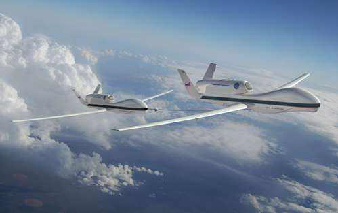
\includegraphics[width=0.75\textwidth]{figures/c01-meaning-1}
  \caption{无人机编队加受油}\label{fig:c01-meaning-1}
 \end{figure}

%\upcite{Takahashi1996Structure,Xia2002Analysis,Jiang1989,Mao2000Motion,Feng1998}%这个是文献引用上标
\section{国内外研究现状及发展趋势}
%\label{sec:***} 可标注label
现如今的无人机自动驾驶仪的结构多为导航模块、位置控制控制模块(外环)以及姿态控制模块(内环);导航模块产生期望位置,位置控制模块由期望位置产生
期望姿态角,姿态控制模块由期望姿态角产生最终的伺服系统的控制量。现如今的低成本无人机所使用的传感器硬件精度比较低,均为消费级别,如果不考虑传感
器的精度问题而设计控制方案,很可能导致整体编队的控制精度下降。现如今已经存在的大部分编队控制算法,未考虑无人机的动力学模型,即只考虑飞机的质点
运动学以及质点动力学条件下提出的导航方法,最终产生的飞行器的控制量为无人机航迹坐标系下的加速度期望值。按照飞机的控制方式,需要将航迹坐标系下的
期望控制量转到机体系之下,但是飞机自动驾驶仪并不能接受加速度控制量,尤其是飞机机体x轴方向,无人机推力、阻力以及重力沿机体方向的推力并非是代数关
系,不能直接由期望加速度得到期望推力;另外由于低成本无人机的惯性原件的精度问题导致无人机不能使用测量的加速度信息作为反馈,两种原因导致以加速度
为最终控制量对于低成本无人机编队的方法控制精度不足。目前的编队控制算法正在向考虑无人机动力学模型方向发展。
|~ : 各章正文内容
\item ~\verb|%%==================================================
%% conclusion.tex for BIT Master Thesis
%% modified by yang yating
%% version: 0.1
%% last update: Dec 25th, 2016
%%==================================================


\begin{conclusion}

本文采用……。{\color{blue}(结论作为学位论文正文的最后部分单独排写,但不加章号。结论是对整个论文主要结果的总结。在结论中应明确指出本研究的创新点,对其应用前景和社会、经济价值等加以预测和评价,并指出今后进一步在本研究方向进行研究工作的展望与设想。结论部分的撰写应简明扼要,突出创新性。)}

\end{conclusion}|~ : 结论
\item ~\verb|\bibliography{reference/chap1}|~ :参考文献
\item ~\verb|%%==================================================
%% app1.tex for BIT Master Thesis
%% modified by yang yating
%% version: 0.1
%% last update: Dec 25th, 2016
%%==================================================


\chapter{***}

附录相关内容…
 |~ : 附录
\item ~\verb|%%==================================================
%% pub.tex for BIT Master Thesis
%% modified by yang yating
%% version: 0.1
%% last update: Dec 25th, 2016
%%==================================================

\begin{publications}{99}

    \item\textsc{高凌}. {交联型与线形水性聚氨酯的形状记忆性能比较}[J].
      化工进展, 2006, 532-535.(核心期刊)
    
\end{publications}
|~ : 攻读学位期间发表论文与研究成果清单
\item ~\verb|%%==================================================
%% thanks.tex for BIT Master Thesis
%% modified by yang yating
%% version: 0.1
%% last update: Dec 25th, 2016
%%==================================================

\begin{thanks}

本论文的工作是在导师……。

\end{thanks}
|~ : 致谢
\item ~\verb|%%==================================================
%% resume.tex for BIT Master Thesis
%% modified by yang yating
%% version: 0.1
%% last update: Dec 25th, 2016
%%==================================================

\begin{resume}

本人…。

\end{resume}
|~ : 作者简介(博士论文需要)
\end{itemize}


\subsection{论文主体文件夹chapters}
\label{sec:thesisbody}

这一部分是论文的主体,是以``章''为单位划分的。

正文前部分(frontmatter):中英文摘要(abstract.tex)。其他部分,诸如中英文信息封
面、授权信息等,都是根据~demo.tex~所填的信息自动生成好了,不需要单独编写文件。

正文部分(mainmatter):是各章内容,在chapter文件夹中。

正文后的部分(backmatter):附录(app\emph{xx}.tex);致谢(thanks.tex);攻读
学位论文期间发表的学术论文目录(pub.tex);作者简介(resume.tex)。参考文献列
表是自动生成的,也不需要作为一个单独的文件。另外,学校的硕士研究生学位论文模
板没有要求加入作者简介,但\textbf{博士的学位论文要求加入作者简介}。


\subsection{图片文件夹~figures}
\label{sec:figuresdir}

figures~文件夹放置了需要插入文档中的图片文件(PNG/JPG/PDF/EPS)。如果图片较多,建议按章再
划分子目录存储图片。

\subsection{参考文献数据库文件夹~reference}
\label{sec:bibdir}

reference~文件夹放置的是各章``可能''会被引用的参考文献文件。参考文献的元
数据,例如作者、文献名称、年限、出版地等,会以一定的格式记录在纯文本文
件.bib中。最终的参考文献列表是BibTeX处理.bib后得到的,名为~demo.bbl。将参
考文献按章划分的一个好处是,可以在各章后生成独立的参考文献,不过,现在看
来没有这个必要。关于参考文献的管理,可以进一步参考第\ref{chap:example}章
中的例子。


\section{进行论文写作}
\label{sec:format}

本节介绍使用论文模板,修改论文信息、摘要、关键字,以及编辑章节等。

\subsection{封面和标题}
在主控文件demo.tex中填写论文的相应信息。

中文封面信息:
\begin{itemize}
\item 中图分类号(\verb|\classification{TQ028.1}|)
\item UDC分类号(\verb|\UDC{540}|)
\item 论文标题(\verb|\title{论文标题}|)
\item 作者姓名(\verb|\author{姓名}|)
\item 学院名称(\verb|\institute{学院名称}|)
\item 指导教师(\verb|\advisor{教授姓名}|)
\item 答辩委员会主席(\verb|\chairman{教授姓名}|)
\item 申请学位(\verb|\degree{学位名称}|)
\item 学科专业(\verb|\major{专业名称}|)
\item 学位授予单位(\verb|\school{北京理工大学}|)
\item 论文答辩日期(\verb|\defenddate{答辩日期}|)
\end{itemize}


英语封面信息:
\begin{itemize}
\item English Title(\verb|\englishtitle{论文标题}|)
\item Candidate Name(\verb|\englishauthor{姓名}|)
\item School or Department(\verb|\englishinstitute{学院名称}|)
\item Faculty Mentor(\verb|\englishadvisor{教授姓名}|)
\item Chair,Thesis Committee(\verb|\englishchairman{教授姓名}|)
\item Degree Applied(\verb|\englishdegree{学位名称}|)
\item Major(\verb|\englishmajor{专业名称}|)
\item Degree by(\verb|\englishschool{Beijing Insititute of Technology}|)
\item The Data of Defence(\verb|\englishdate{答辩日期}|)
\end{itemize}

\subsection{摘要和关键字}
摘要内容,放置于chapters文件夹下的abstract.tex中,

中文摘要于\verb|abstract|环境编写;\verb|\keywords|为中文关键字。英文摘要于\verb|englishabstract|环境编写;\verb|\englishkeywords|为中文关键字。

\begin{lstlisting}[language={[LaTeX]TeX}, caption={ 中英文摘要 }]
\begin{abstract}
	本文 ...
\keywords { 形状记忆;聚氨酯 }
\end{abstract}

\begin{englishabstract}
   In order to exploit ...
\englishkeywords{shape memory properties; polyurethane}
\end{englishabstract}
\end{lstlisting}


\subsection{正文章节}
章节的设置分别通过关键字完成,按照章节的级别依此如表~\ref{tab:setSection}所示,关于文档中具体章节的关键词设置可以参看原宏包中tex文件夹下的实例文件。

\begin{table}[htb]
 \centering
  \caption{章节设置关键字}     % title of Table
  \label{tab:setSection}    % label of Table
  \begin{tabular}{cl}
    \hline
    章节级别        & 关键字     \\
    \hline
     章        & \verb|\chapter| \\
     节        & \verb|\section | \\
    子节      & \verb|\subsection |\\
    表格名称       & \verb|\caption{标题名称}| \\
    引用标签       & \verb|\label{引用名称}| \\
    \hline
  \end{tabular}
\end{table}

\subsection{其他部分}


全文总结、攻读学位期间发表论文与研究成果清单、致谢的内容,均位于chapters文件夹下,分别为conclusion.tex,pub.tex,thanks.tex。

\section{交叉引用}
\subsection{公式、图表和插图引用}
\label{sec:refofFigAndTab}
交叉引用的前提是需要在定义章节、公式和图表的时候都对其进行命名标签(即\textbackslash label\{sec:labelName\}命令),在实际使用过程中通过标签进行引用。根据引用的特点可以将应用分成表~\ref{tab:citeType}中所示三类。

\begin{table}[htb]
 \centering
  \caption{交叉引用类型}       % title of Table
  \label{tab:citeType}    % label of Table
  \begin{tabular}{cl}
    \hline
    引用类型     & 关键字     \\
    \hline
    标签设置        & \textbackslash label\{marker\}  \\
    引用代号        & \textbackslash ref\{marker\}    \\
    引用页码        & \textbackslash pageref\{marker\} \\
    引用文献        & \textbackslash cite\{regLabel\} \\
    \hline
  \end{tabular}
\end{table}

其中,表格和图片的摆放位置由 \textbackslash begin\{table\}或\textbackslash begin\{figure\}后面的中括号设置,例如[htb]表示可以将图表放在当前位置(here)、页面顶端(top)或者页面底端(bottom)。

{\bf{实例1:}}这里是对表格《交叉引用类型》的引用——表~\ref{tab:citeType}位于第~\pageref{tab:citeType}页,其标签为\textbackslash label\{tab:citeType\}。


\subsection{文献引用}
\label{sec:citeRefs}

BIT-Thesis论文模板使用BibTeX处理参考文献。

参考文献的具体内容就是reference文件夹下的chap\textit{xx}.bib,参考文献的元数据(名称、作者、出处等)以一定的格式保存在这些纯文本文件中。
.bib文件也可以理解为参考文献的``数据库'',正文中所有引用的参考文件条目都会从这些文件中``析出''。

正文中引用参考文献时,用\verb+\upcite{...}+可以产生“上标引用的参考文献”,
如\upcite{chen2007act},\upcite{Meta_CN,chen2007act,DPMG}。

具体使用方法参见第\ref{sec:reference}节。
